% Setup - do not change
\documentclass[11pt]{article}
\usepackage[top=0.9in, left=0.9in, bottom=0.9in, right=0.9in]{geometry} 
\usepackage{parskip}

\usepackage[english]{babel}
\usepackage[utf8]{inputenc}
\usepackage{amsmath,amsthm,amssymb,graphicx,pdfpages,lipsum,hyperref}
\usepackage[none]{hyphenat}
\usepackage{csquotes}

\setlength\parindent{0pt}
%%%%%%%%%%%%%%%%%%%%%%%%%%%%%%%%%%%%%%%%%%%%%%%%%%%%%%%%%%%%%%%%%%%
% add other packages here if required

%% Bibliography are specified in this file. You can also choose inline bib style if you want to. But make sure your citation style is consistent (and proper)
% For more details on citation: https://library.unimelb.edu.au/recite
\usepackage[sorting = none]{biblatex}
\usepackage{multirow}
\usepackage{booktabs}
\usepackage[inline]{enumitem}
\usepackage{multicol}
\usepackage{afterpage}
\usepackage{subcaption}
\usepackage[font=small,labelfont=bf,tableposition=top]{caption}

\addbibresource{references.bib}

%%%%%%%%%%%%%%%%%%%%%%%%%%%%%%%%%%%%%%%%%%%%%%%%%%%%%%%%%%%%%%%%%%% the '%' symbol denotes comments

% Begin document creation
% DELETE THE \lipsum PLACEHOLDERS WHEN YOU BEGIN
\title{\textbf{Predicting Hourly Demand for Taxi Rides in NYC}}
\author{
Ming Hui Tan \\
Student ID: 1087948\\
%% Replace the link with your github repo
% 1. Remember to escape underscore (\_) in the link.
% 2. Remember to include the commit you want to submit in the link
\href{https://github.com/MAST30034-Applied-Data-Science/mast30034-project-1-olivertan1999}{Github repo with commit}
}

\begin{document}
\maketitle

\section{Introduction}
% Link to a 30 min tutorial if you require revision: https://www.overleaf.com/learn/latex/Learn_LaTeX_in_30_minutes
The traditional street-hailing taxi systems in metropolitan cities are often deemed inefficient due to the low ratio of \textit{live miles} (miles spent with fare) to \textit{cruising miles} (miles spent without fare) \cite{inproceedings}. On top of that, with the recent rise in inflation, higher fuel costs continue to put taxi drivers in a desperate position to reduce their cruising miles. However, with the deployment of networked sensors, large amount of information such as GPS traces, pick-up and drop-off time, number of passengers, weather etc. can be collected and processed to develop an intelligent dispatch system that provides systematic routing for taxi drivers in advance to meet local passengers demand. 

In this paper, we will present two different Machine Learning approaches and evaluate their efficacy in estimating hourly passengers demand for taxi rides around New York City (NYC). Besides benefiting taxi companies and drivers, the outcome of this paper could be extended to support decision makings among public agencies in urban developments.

Throughout this paper, we use the hourly count of pick-ups to represent the hourly taxi demand in a region. Despite using met taxi demand data, the outcome of our prediction will paint a general picture of the overall demand in a region for which unmet demand can then be inferred from.  

\subsection{Dataset}
The main data set chosen for this paper is the \textbf{TLC Taxi Trip Record Data} published by the NYC Taxi \& Limousine Commission, which includes trip records (time and location of pick-ups and drop-offs, fare amount, etc.) from all trips completed in yellow and green taxis in NYC \cite{tlctriprecorddata}. Due to various travel restrictions and how the pandemic has changed the lifestyles of the residents and travellers in NYC, we assume that the trip records before 2021 will no longer reflect the actual demand today. Therefore, we decided to use the latest data available from October 2021 to April 2022 for our modelling and analysis.

In addition, external data sets including the \textbf{Primary Land Use Tax Lot Output (PLUTO)} published by the NYC Department of City Planning \cite{plutodata} and the US National Center for Environmental Information's \textbf{Integrated Surface Data} collected at Central Park, NY \cite{noaadata}, were used to supplement our analysis. 

The PLUTO data set details information about every piece of land in the city including their number of units, lot sizes as well as the building classes for each lot. On the other hand, the Integrated Surface dataset provides detailed representation of the hourly weather conditions through features such as the temperature and dew point of the region. These external datasets were selected as we expect that there are weather and geographical links with the hourly demand in specific regions in NYC. 

The basic summary of the data sets after adjusted to the required period is as follow


\begin{table}[h]
\begin{center}
    \begin{tabular}{lcc}
        \toprule
        \bf Datasets & \bf Instances & \bf No. features\vspace{0.1mm}\\
        \hline
        \vspace{-0.1mm}TLC Yellow Taxi Trip Record Data & 22,821,986 & 19\vspace{0.1mm}\\
        \hline
        \vspace{-0.1mm}TLC Green Taxi Trip Record Data & 605,645 & 20\vspace{0.1mm}\\
        \hline
        \vspace{-0.1mm}Primary Land Use Tax Lot Output& 856,977 & 91\vspace{0.1mm}\\
        \hline
        \vspace{-0.1mm}NCEI Integrated Surface Dataset & 6691 & 94\\
        \bottomrule
    \end{tabular}
    \caption{Datasets shape}
    \end{center}
\end{table}
\vspace{-3mm}
\section{Preprocessing}
Various preprocessing steps were done on the three data sets to ensure that they follow the expected structure. The following section will detail the inconsistencies found in each data sets and how we processed them.
\subsection{Data Wrangling and Feature Selection}

\subsubsection{TLC Trip Record Data}
Due to the sheer amount of data (totalling \textcolor{red}{23,427,634} rows), we found that there were several issues in the data that were either inconsistent with our research requirements or just purely entry errors. The following steps were taken to resolve such inconsistencies:
\begin{itemize}
\item \textbf{Records not within the defined date range} were removed to fit our research requirement.\vspace{-1mm}

\item \textbf{Negative amount for fare, tips and other fees-related columns} were found in the data and trips containing these were discarded entirely as invalid records. In the end, only records with fare amount greater or equals to \$2.50 were included as this is the initial fare amount for any ride according to the TLC webside.
\vspace{-1mm}

\item \textbf{Negative or extremely short trip distance} were found in certain records and they were discarded as well. Only records with greater or equals to 0.5 miles were retained as we assume that rational consumers would rather walk than take the cab if the distance to destination is short especially in the cities where traffic congestion is a major issue.
\vspace{-1mm}

\item \textbf{Negative trip-duration} records, where the drop-off time is earlier than the pick-up time, were discarded as invalid or purely entry errors. Only records with trip duration longer than a minute were retained as we assume that rational passengers would not be willing to pay the initial \$2.50 fare for a ride that takes less than a minute.
\vspace{-1mm}

\item \textbf{Negative or zero passenger count} was found in certain records and these were removed as invalid records in the data. 
\vspace{-1mm}

\item \textbf{Trips with pick-up destination located outside the defined region} were also removed as we are only interested with demand within NYC. These are records with Location ID outside the predefined range of 1-263.

\item \textbf{Extreme values in trip distance, trip duration and fare-related fields} were found in a small portion of the records. The statistical method involving using interquartile to discard outliers would erase too much of our data. Instead, we discovered that the 99.99th percentile of the data were still logical and possible for each of the specified columns. For example, the highest fare amount was \$259 which is possible given that the longest trip distance was about 66 miles when we filtered to the 99.99th percentile for both fields. Since our research revolves around the number of hourly pick-ups, our analysis would not be sensitive to the figures in these fields. Nonetheless, highly unrealistic records such as 6 figures value for trip distance were removed to ensure the overall quality of the data set.
\end{itemize}

In total, we removed 2,867,171 entries ($\approx12.24\%$) of our original TLC data set, leaving \textcolor{red}{20,560,463} remaining instances in total for our modelling and analysis. Most of the features mentioned above except date, time and location related features, were not included in our modelling and analysis in Section \ref{analysis} as they were trip-specific and we would not have these data available when predicting future hourly demand. However, as mentioned before, data wrangling involving these fields was necessary to preserve the quality of the data set.



\subsubsection{Primary Land Use Tax Lot Output}
The overall dataset has a large number of features totalling 91. However, a large portions of them were either not informative for our modelling purpose or contain large proportion of missing values. Examples of such features are building heights, lot area and owners' name. As the data set was retrieved using the NYC Open Data Api, we were able to obtain the subset of features through simple querying. The selected features are:

\begin{multicols}{3}
\begin{itemize}
  \item Latitude and Longitude
  \item Building Class
  \item Zipcode
  \item Borough
  \item Total Units
  \item Total Residential Units
\end{itemize}
\end{multicols}
To integrate the data into our analysis, we spatially joined the PLUTO data set with the TLC Zone data set, which details the locations of the trip records, using the ``within'' method in the \textit{sjoin} function under the geopandas library. This allowed us to match any buildings located within each specified location ID in the TLC Zone data based on their latitude and longitude, as well as discard any buildings outside the specified zones. In the end, 3,438 buildings were discarded, leaving \textcolor{red}{853,539} remaining records in the data set.

\subsubsection{NCEI Integrated Surface Dataset}
The preprocessing of the Integrated Surface data set was more involved as the data were presented with multiple values separated with commas within each element. Furthermore, the values were scaled with factors specific to each field. With the help of the data dictionary provided, we were able to extract and unscale the values accordingly. Similar to the PLUTO data set, the Integrated Surface data set also contained a large number of features of which, a large proportions of them were mostly missing values. Thus, these features were discarded and the following features were retained:
\begin{multicols}{3}
\begin{itemize}
  \item Date and Time
  \item Wind Speed
  \item Temperature
  \item Dew Point
  \item Atmospheric Pressure
\end{itemize}
\end{multicols}
We then filtered the dates in the data from the 1st of October 2021 to the 31st of April 2022 to match our research period. There were also very few missing values in the selected features. Instead of discarding them and potentially losing weather information for a few specific hours, we decided to impute the missing value with the data from previous hour. 

\subsection{Feature Engineering and Data Aggregation}
For the TLC Trip Record Data, we extracted the pick-up date and hour into individual columns. We then grouped the data based on pick-up location ID, date and hour to count the number of instances as the representation of our hourly demand in the region. We also generated a feature to specify if the date is a weekend/public holiday and extracted the day of week as we expect strong temporal patterns associated with taxi rides demand.

With the processed PLUTO data set, we aggregated the data based on location ID and counted the number of buildings based on their building classes in that region. We then included this information in the TLC Zone data set such that for each location ID in the TLC Zone data set, there are columns for each building class that detail the number of building under that specified class. Finally, we joined the modified TLC Zone data set with the TLC Trip Record Data using inner join on location ID. We also merged the resulting data set with the Integrated Surface data set on date and hour.

\section{Preliminary Analysis}
\label{analysis}
In this section, we explored the features in TLC data set individually as well as their relationship with the PLUTO and weather data sets. 

\subsection{Distribution of Pick-ups Demand}
Based on our analysis, we discovered that the distribution of taxi demand has a strong correlation with the Location ID. From Figure \ref{fig:label}, we can clearly see that the average daily pick-up activities are concentrated around Manhattan and the three main airports in NYC (Newark Liberty International, LaGuardia and John F. Kennedy International) with a total of 18,445,440 million trips ($\approx89.7\%$ of the total trips) and 87,000 average daily trips done in Manhattan alone during this period. Due to the skewness of the data, we plotted the log average daily demand instead to scale down the data for a more meaningful comparison.
\begin{figure}[h]
    \centering
    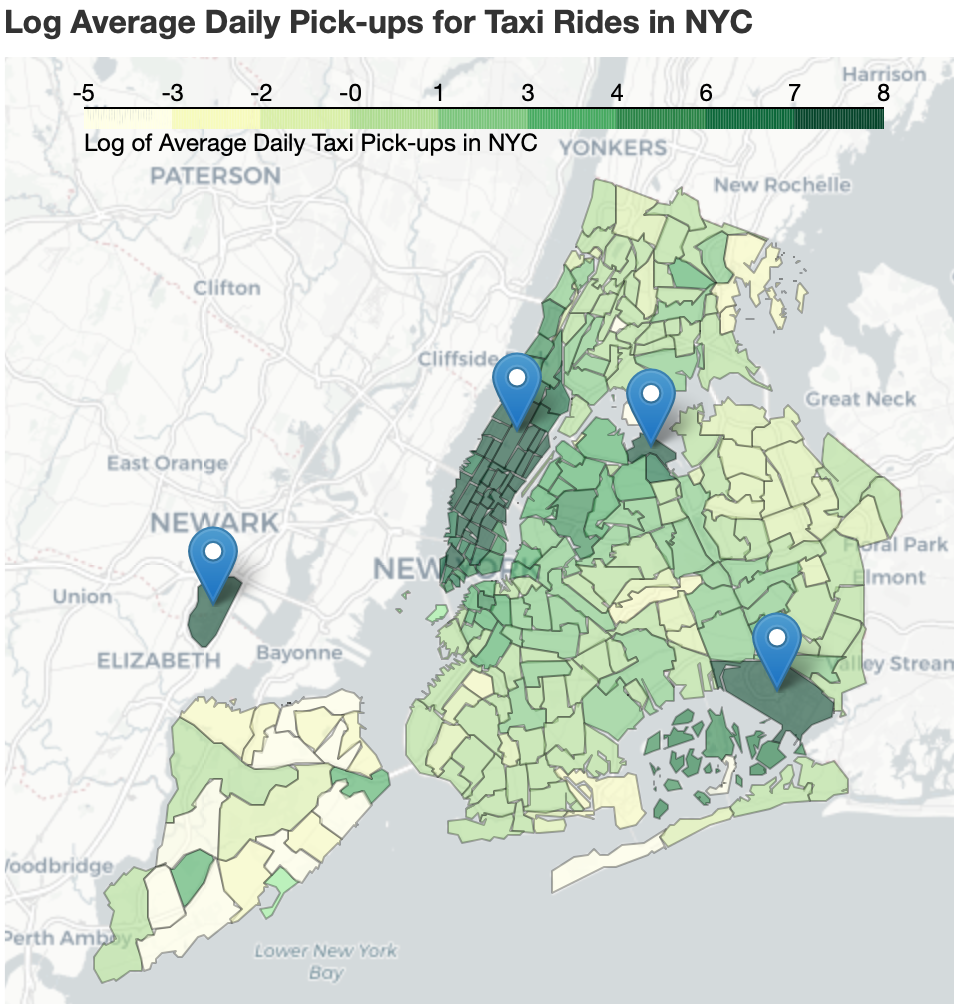
\includegraphics[width=3.2in, height=3.2in]{plots/location_pickup.png}

    \caption{Distribution of Average Daily Pickups in NYC}
    \label{fig:label}
    
\end{figure}
\subsection{Trend of Taxi Rides Demand}
Besides location, we also observed strong temporal patterns in the taxi demand. In Figure \ref{fig:sub1}, there are clear cyclical patterns in the daily taxis pick-up. The trend seems to be pretty consistent overall except for the period between December and February, where the demand seems to be on the lower end consistently. This is likely due to the impact of major federal year-end holidays (indicated by yellow lines in Figure \ref{fig:sub1}) such as Christmas and New Year's Day, where most people are not obligated to go to work, resulting in sharp decline for demand during these periods.

Interestingly, the sharpest decline happened on 29 January 2022 (indicated by the red line in Figure\ref{fig:sub1}). Upon further research, we found out that a major blizzard hit the city on this particular day and several states in the US declared emergencies in response to the storm \cite{blizzard}, which explains the plummet in taxi demand during this period. This led us to believe that weather also holds a significant influence over the taxi demand. 

Looking further into the hourly pick-ups of different days of the week in Figure \ref{fig:sub2}, there are obvious differences in the hourly trends between weekdays and weekends. For instance, after 5 am, there seems to be a spike in demand on weekdays which is likely contributed by workers getting to their workplaces. On weekends, however, this spike happens hours later which is most likely due to people getting up later on a weekend. In addition, the hourly pickups on weekdays also exhibit identical pattern between one another. Overall, these time-series plots strongly suggest that the day of the week as well as public holidays have a strong influence on demand in NYC.

\begin{figure}[h]
\centering
\begin{subfigure}{.5\textwidth}
  \centering
  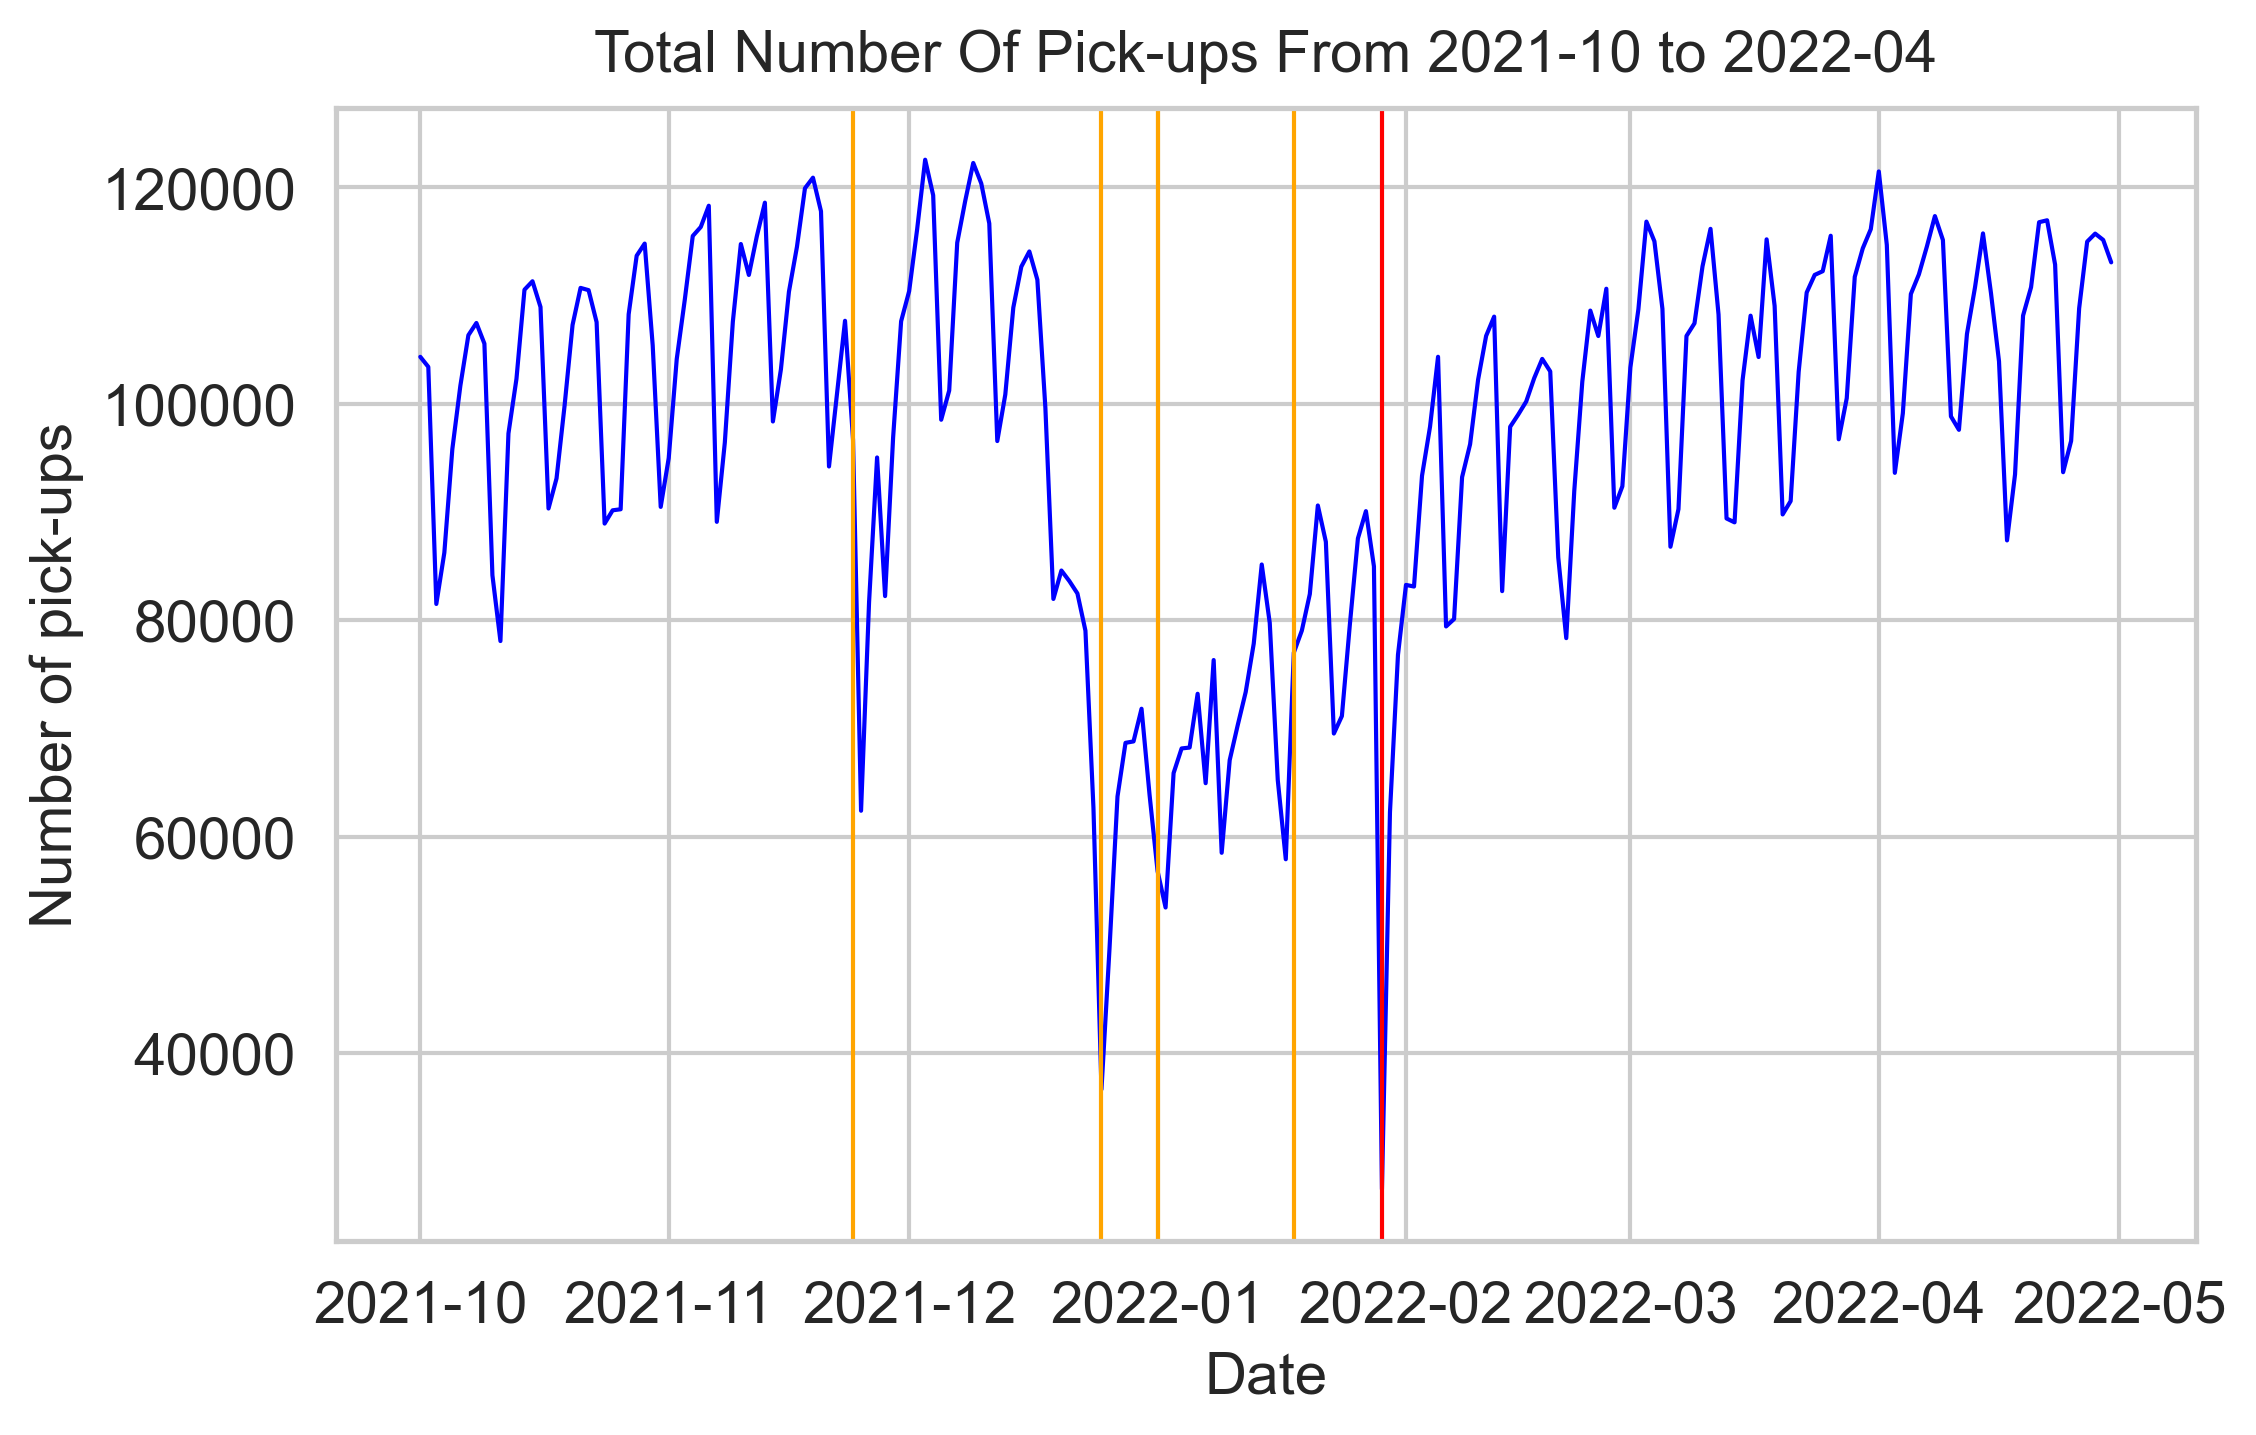
\includegraphics[width=1\linewidth]{plots/trend.png}
  \caption{Total Daily Demand}
  \label{fig:sub1}
\end{subfigure}%
\begin{subfigure}{.5\textwidth}
  \centering
  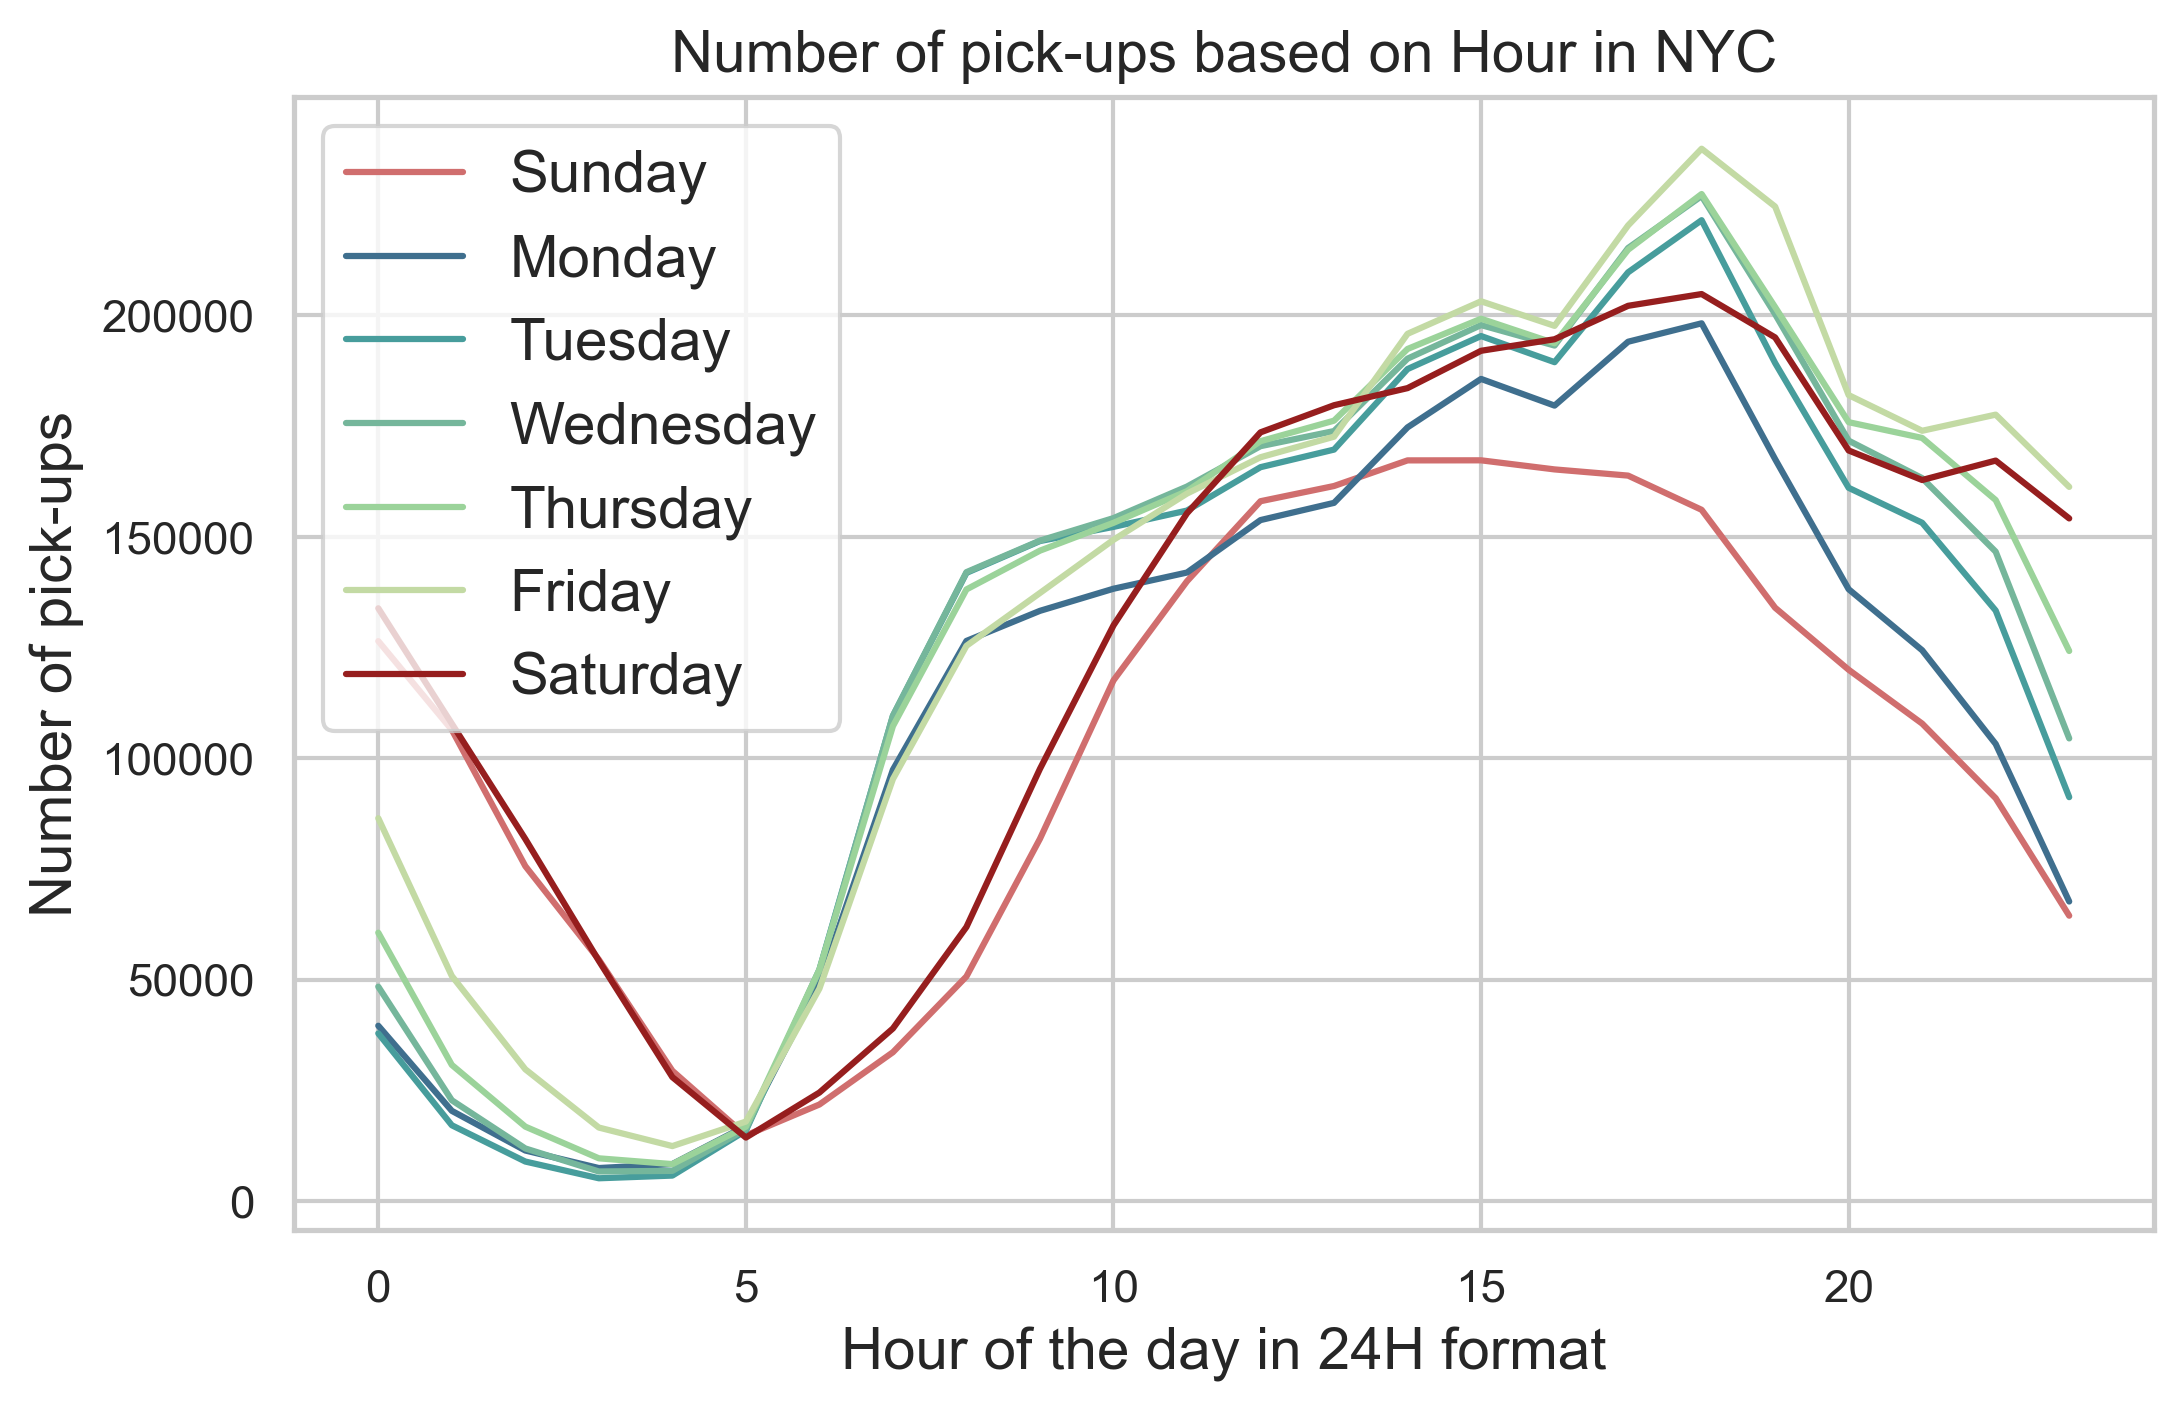
\includegraphics[width=1\linewidth]{plots/hourly_trend.png}
  \caption{Total Hourly Demand}
  \label{fig:sub2}
\end{subfigure}
\caption{Taxi Rides Demand Trend}
\label{fig:hotel_trend}
\end{figure}
\vspace{-3mm}
\subsection{Effect of Buildings Classes on Pick-up Demand}
Out of all 24 building classes, only the `Hotel' building class exhibits a visible upward trend with the average daily demand (with \textit{Pearson correlation coefficient} of 0.33) as shown in Figure \ref{fig:hotel_trend}. This makes perfect sense since most travellers who stay in hotels likely lack personal means of transport. Thus, they will resort to alternatives such as taxi rides or public transports to get to their destinations. Hence, locations with more hotels will attract greater demand for taxi rides.
\vspace{-2mm}
\begin{figure}[h]
    \centering
    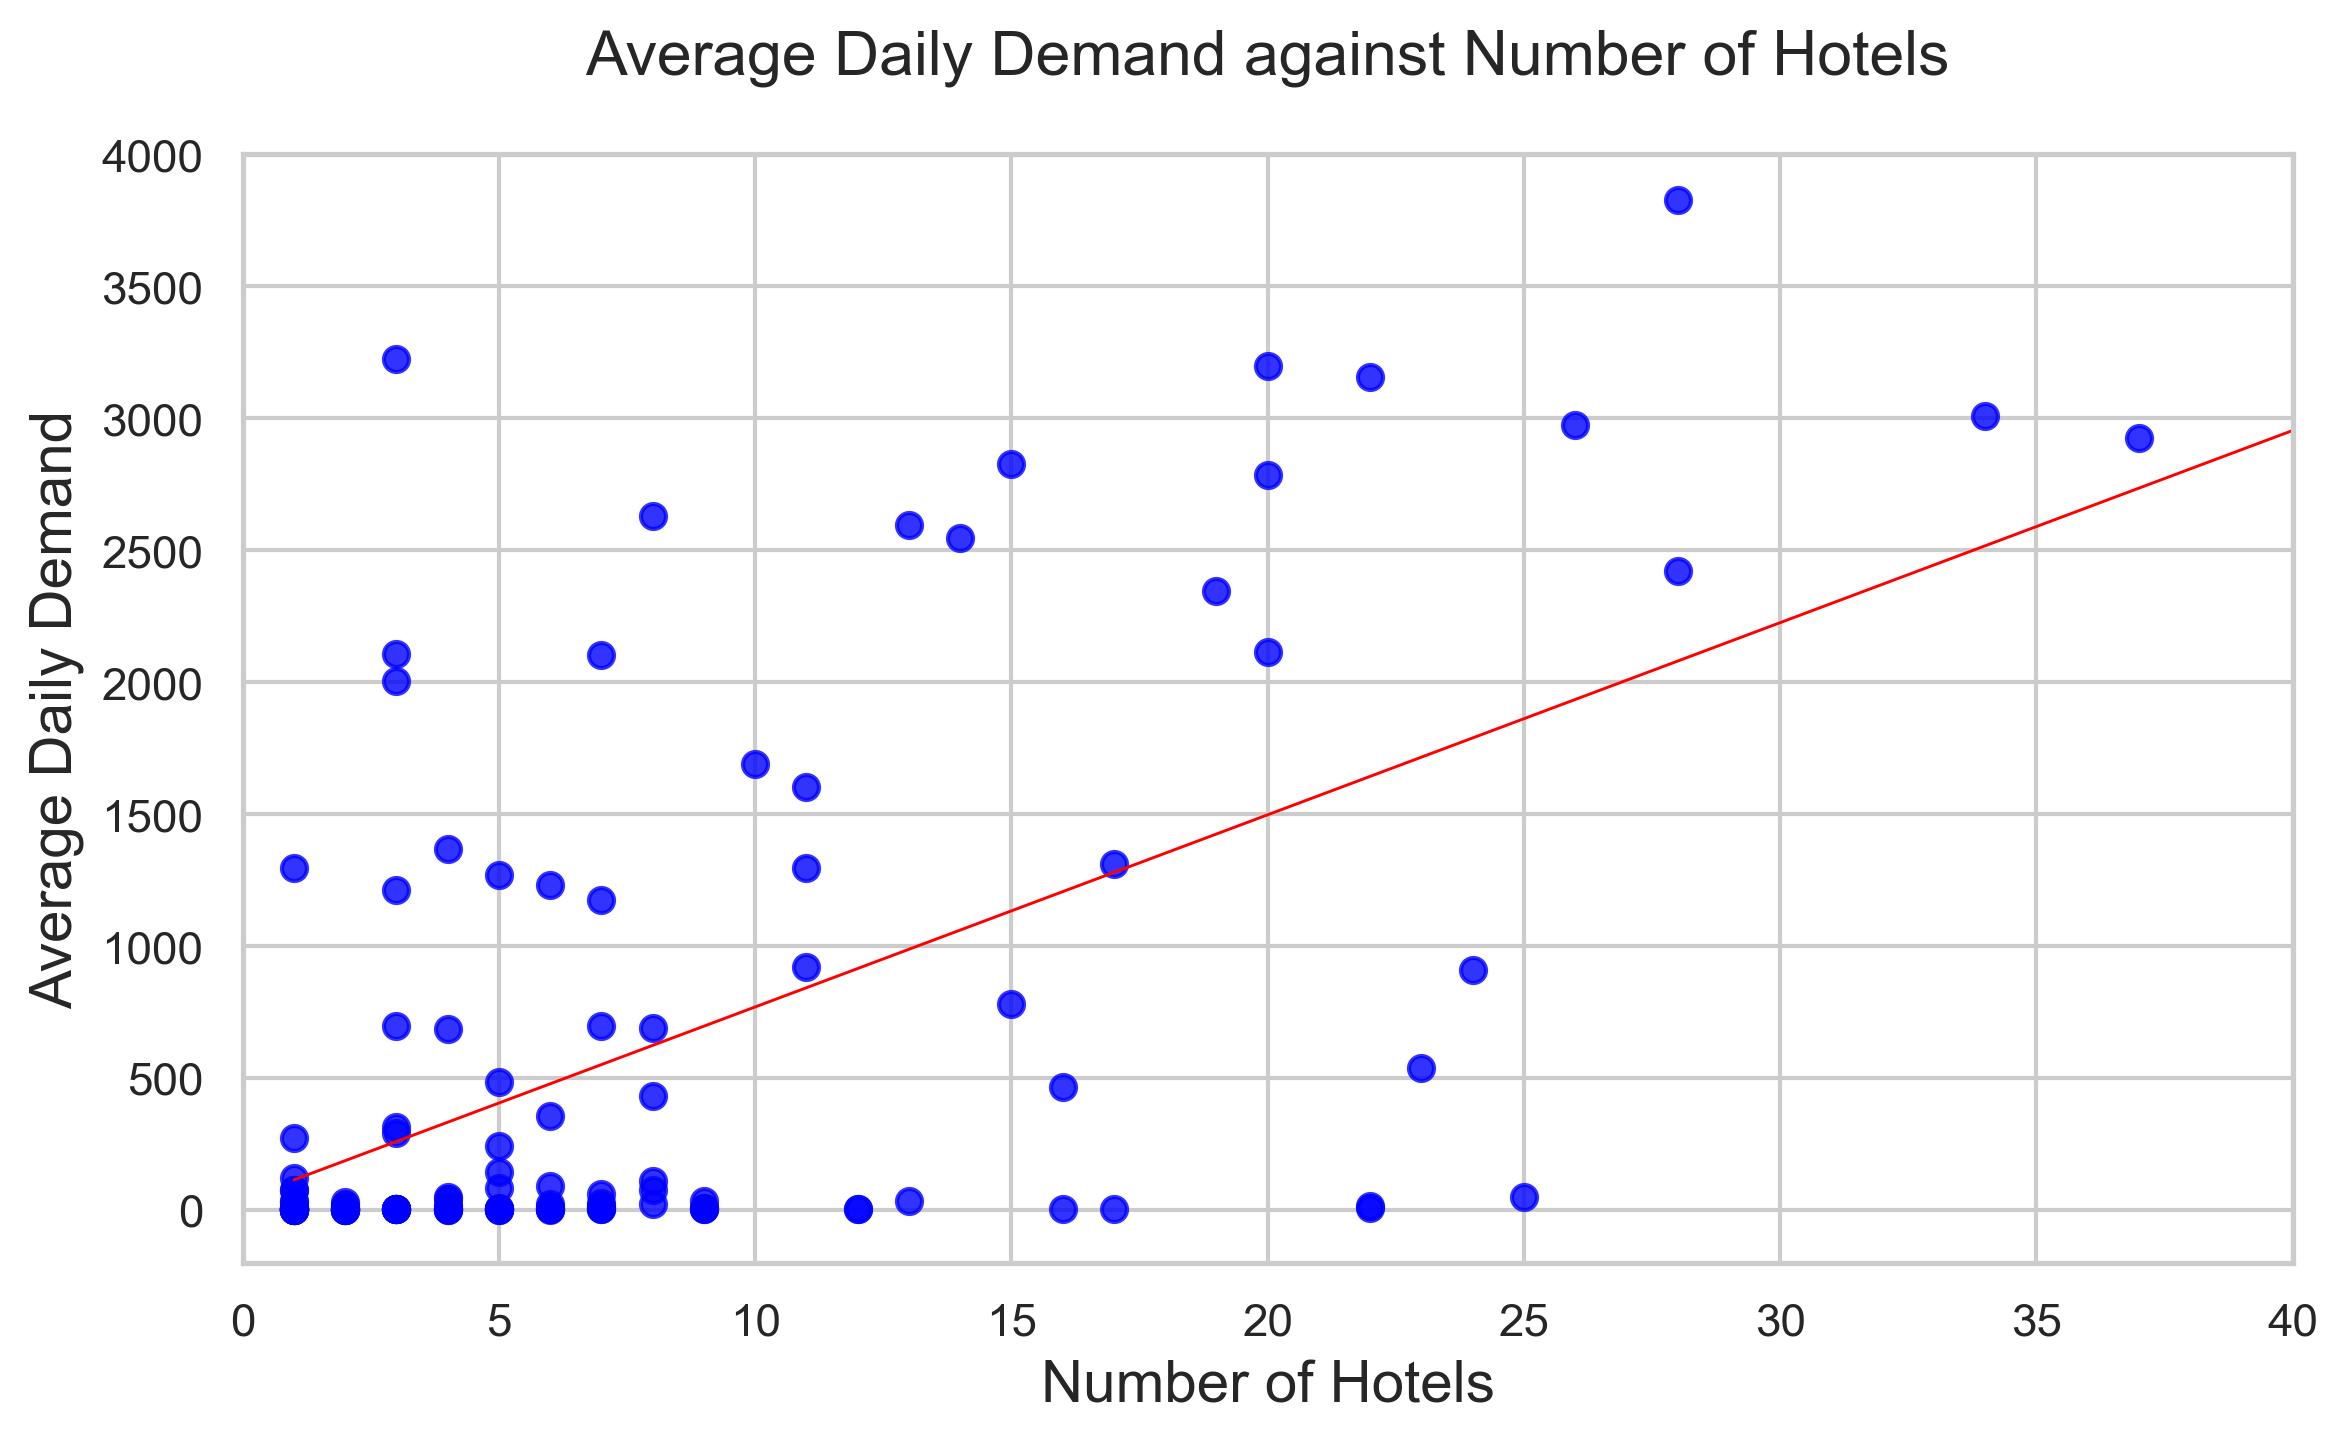
\includegraphics[width=5in, height=3in]{plots/hotel_on_pickup.png}

    \caption{Average Daily Demand for Taxi by Number of Hotels in the Pick-up Location in NYC.}
    \label{fig:hotel_trend}
\end{figure}


\section{Modelling}
Two different regression models, namely \textit{Linear Regression (LR)} and \textit{Random Forest Regression (RFR)}, were implemented to evaluate their performance on predicting the hourly taxi rides demand in NYC.

Due to the skewness and the volume of the data set, we decided to train each model on the 6 different boroughs separately as this will retain the relevant information about each borough in each model. In addition, to predict future demand, we assumed that forecast weather information will be available in advance. We also assumed that we would also have information about which borough we are predicting and the building information in each location does not change hourly. Finally, we trained the models on the first 5 months data (October 2021 to March 2022) and evaluated the model on the April 2022 data. To ensure that we have a fair comparisons between the models, we decided to use the same predictors for both models. 

\subsection{Linear Regression}
Since we are predicting a numerical output using both categorical and numerical predictors, regression methods such as LR is capable of the task \cite{linearregression},\cite{linearstatsmodel}. In our model, we assumed no interactions between the categorical variables in the linear models considering every day has the same number of hours and the location does not depend on the date or time and vice versa. Thus, we have the following model:
$$Y_{ijklm}=\mu+\alpha_i+\beta_j+\gamma_k+\delta_l+\xi_m+\sum_{s=1}^{p}a_sX_s+\epsilon_{ijklm}$$
where $\alpha_i$ are the main effects for location, $\beta_j$ are the main effects for month, $\gamma_k$ are the main effects for day of the week, $\delta_l$ are dummy variable to indicate a weekday or weekend and $\xi_m$ are the hours in a day. The remaining $\{X_1,X_2,...,X_p\}$ are the additional numerical predictors consisting of weather information and the number of buildings in the location based on the building classes.

\subsection{Random Forest Regression}
The RFR is a supervised learning algorithm that aggregates multiple decision trees built on bootstrapped samples of the training data for regression. This ensemble learning method allows the RFR model to reduce the high variance problem frequently associated with using a single decision tree and improve overall prediction accuracy \cite{randomforest}. The RFR model performs well on features with non-linear relationship but its downfall lies on its interpretability. However, since taxi drivers would not be much interested in the interpretability of the result rather than the accuracy, we decided that RFR would be a suitable model for the task.

To tune the hyperparameters of our RFR model, we ran a cross-validated grid search on a set of parameters with the entire training data to approximate the most optimal configurations for the model for each borough. We were unable to run the grid search individually on each borough's model due to limited computational time.

\section{Results and Discussion}
To evaluate our models, we used the Root Mean Squared Error (RMSE) as our loss metric since it is highly interpretable and it allows us to contextualise the errors of the models and their implications in predicting future taxi demand. Table 2 demonstrates the performance of the model based on each borough in NYC.

\vspace{0.5cm}
\begin{minipage}{\textwidth}
  \begin{minipage}[b]{0.5\textwidth}
  \centering
  \begin{tabular}{lcc}
  \toprule
    \multirow{3}{*}{} &
      \multicolumn{2}{c}{\bf RMSE} \\
      \cmidrule(lr){1-3}
      \bf Borough & \bf LR & \bf {RFR} \\
      \midrule
    Manhattan & {44.98} & {\bf 20.45} \\
    \hline
    Queens & {33.72} &  \bf 16.07 \\
    \hline
    Brooklyn & { 1.80} & \bf 1.59 \\
    \hline
    Bronx &  {\bf 0.58} & \bf 0.58\\
    \hline
    Staten Island &  {1.49} & \bf 1.46\\
    \hline
    EWR &  {\bf15.24} & 16.96\\
    \bottomrule
    
  \end{tabular}
    %   \vspace{-5mm}
      \label{Table2}
      \captionof{table}{Performance of the models on the \\test set}
      \vspace{-0.3cm}
    \end{minipage}
  \hspace{-0.8cm}
  \begin{minipage}[t]{0.5\textwidth}
  \captionsetup{justification=centering}
    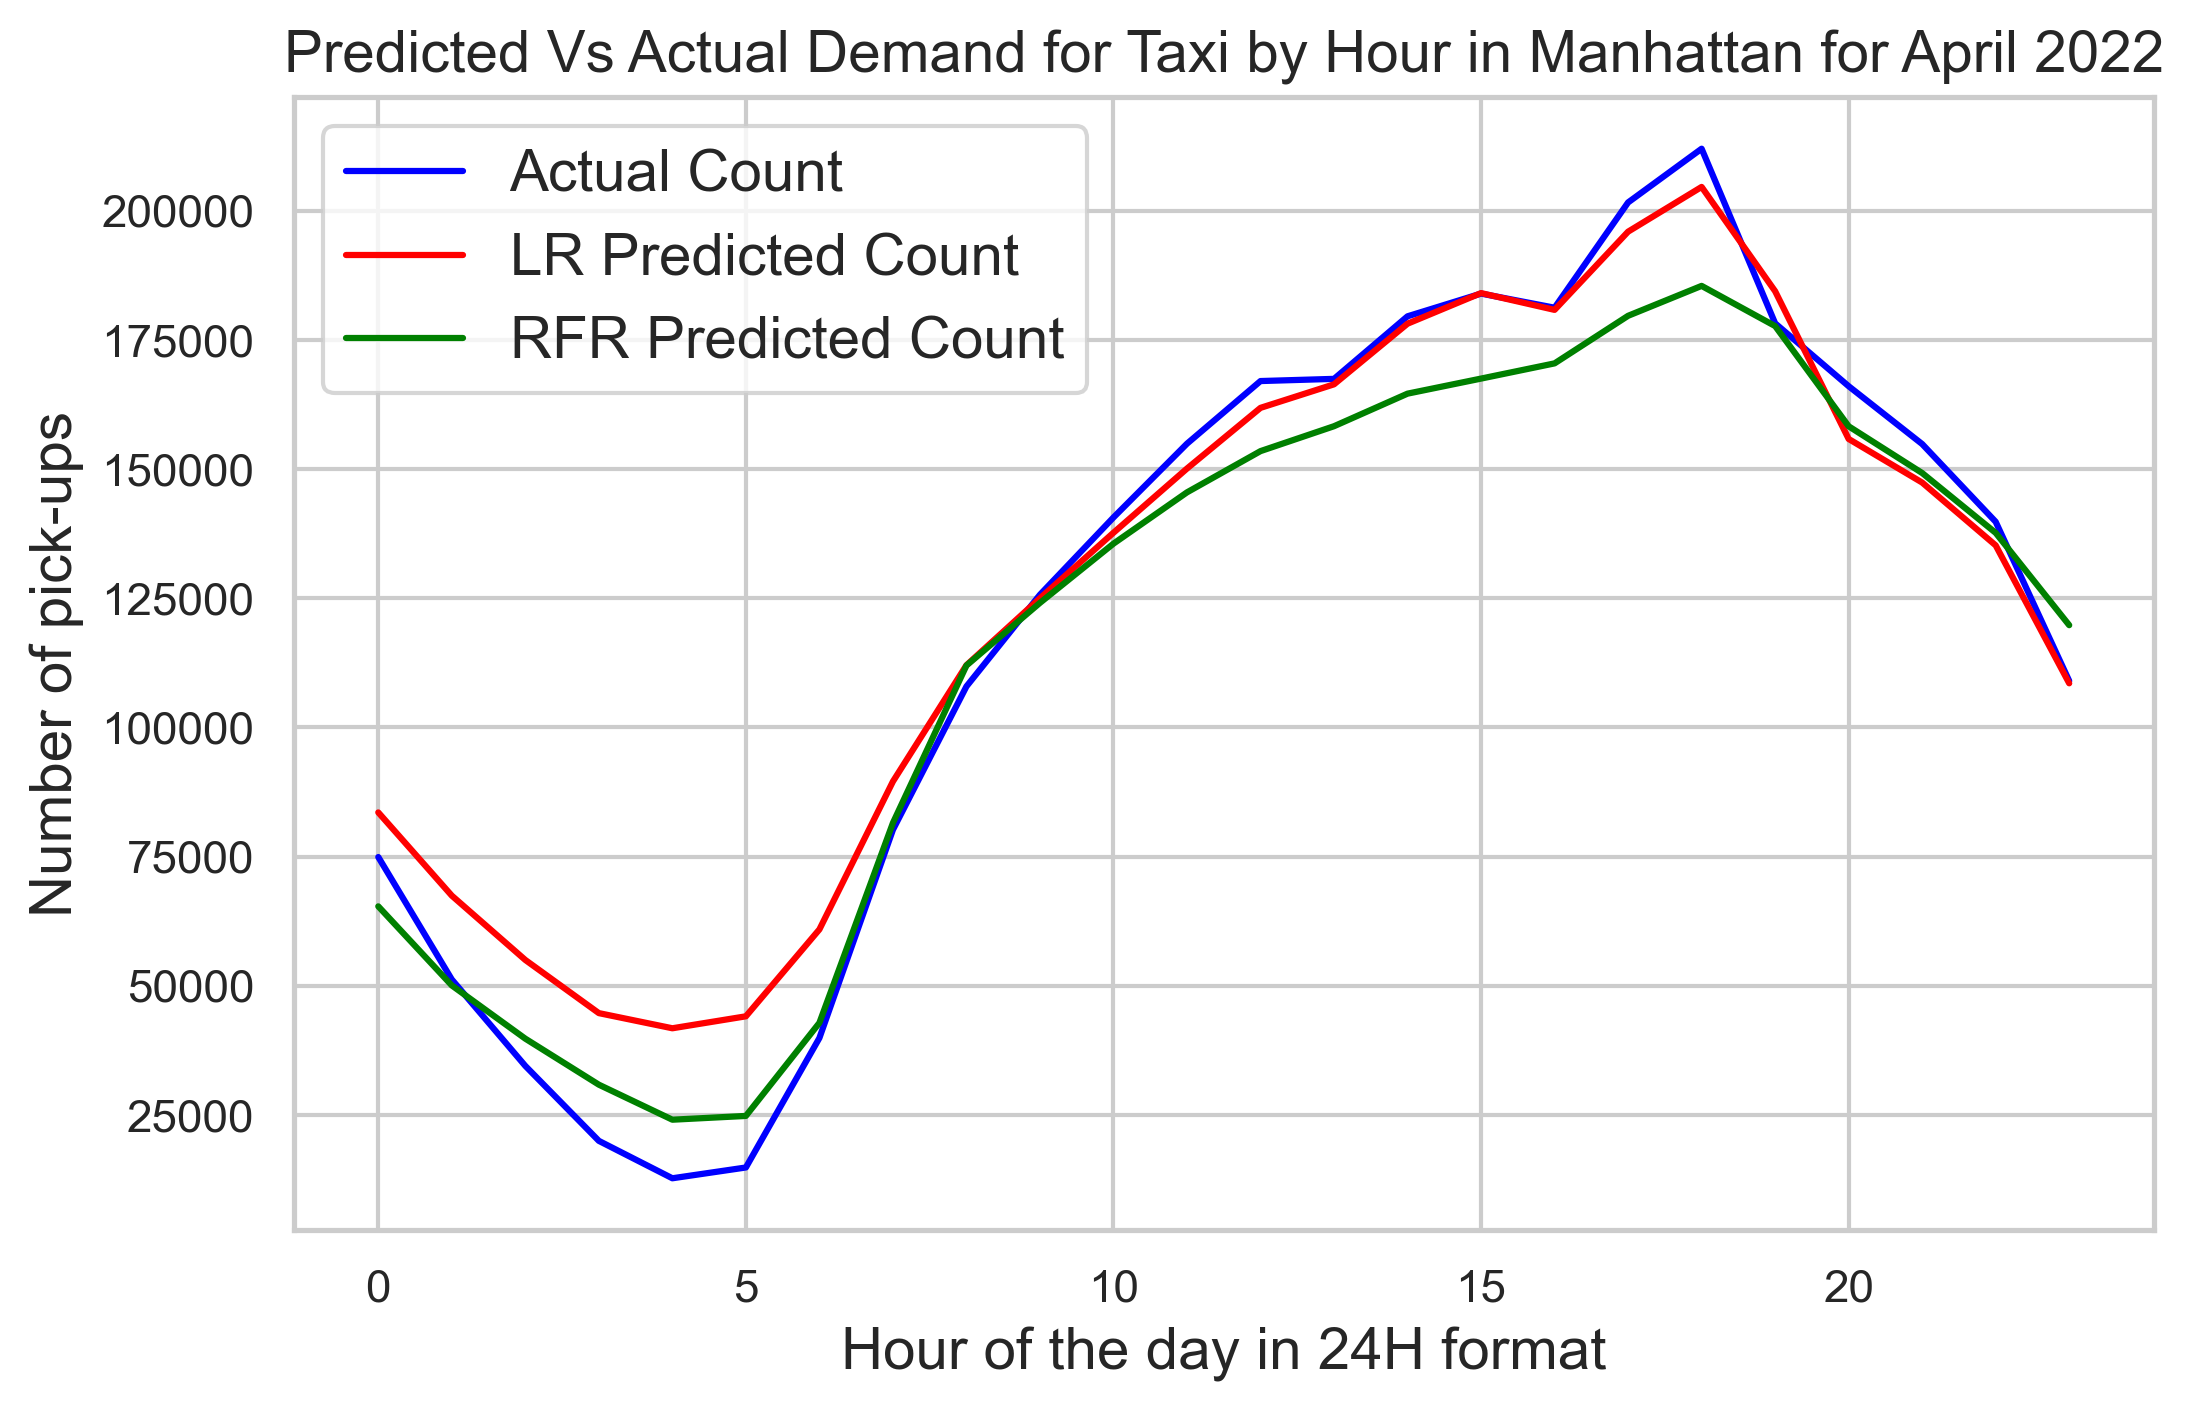
\includegraphics[width=1\linewidth]{plots/predicted_trend.png}
    
    \vspace{-0.3cm}\captionof{figure}{Actual vs Predicted Pick-ups in Manhattan for April 2022}
    \label{fig4}
  \end{minipage}
  
  \end{minipage}
\vspace{0.3cm}

Based on Table 2, it appears that RFR dominated LR in almost every borough's test set. However, despite the high RMSE in LR, the model was still able to predict very closely to the actual demand in Manhattan after around 8 am as shown in Figure \ref{fig4}. This could be a sign of overfitting as there were significantly more records of data after 8 am and LR is highly prone to overfitting especially with large feature space. Therefore, LR was able to predict accurately for popular locations during peak period in Manhattan but fail to generalise to locations or period with sparse demand, hence the high RMSE value.

On the other hand, RFR showed consistent performance in predicting hourly taxi demand for both popular and less popular locations since it is less prone to overfitting than LR. This explains how the model was able to achieve lower RMSE value despite Figure \ref{fig4} showing LR being much closer to the actual count after 8 am. The model was also able to learn non-linear relationships and discover interactions between features in the data where LR was able to.

Both models seemed to overestimate the number of pickups before 8 am, while underestimating the demand during peak hours (10 am - 6 pm). However, considering the low RMSE of RFR, the model will still be effective in predicting the general hourly demand for taxi in various locations in NYC. LR, however, showed signs of overfitting and high RMSE, suggesting that the model might not be suitable for the task.


\section{Recommendations}
Based on our model evaluation, we can clearly see that the RFR model is very effective in estimating the hourly demand for taxi rides in NYC with an average error of only about 20 trips in Manhattan and much less for other boroughs. Considering the hourly demand can reach up to 900+ in popular destinations in Manhattan, this puts in perspective on how low the average error is and overall how accurate the model is.

Therefore, we recommend firms in the industry to look into producing and refining such model with their own internal data sets to develop an intelligent dispatch system with accurate and relevant hotspots predictions to inform and ease the routing of their taxi drivers. This would not only benefit the taxi drivers by lowering their cruising miles and effectively reducing their cost of operations, it may also increase the drivers' retention rate and potentially raise the profitability for both the drivers and the firm. 

As for taxi drivers, based on previous analysis in Section 3, we highly recommend frequenting locations in Manhattan where many hotel buildings are located at. This is based on the evidence of an upward trend between number of hotel buildings and demand for taxi rides as shown in Figure \ref{fig:hotel_trend} as well as the popularity of taxi rides in Manhattan depicted in Figure \ref{fig:label}. Alternatively, drivers could cruise the three main airports as they are also part of the major hotspots in NYC. Since the demand for taxi is high in these regions, drivers could manage their routes around these regions to increase their likelihood of picking up passengers and effectively reduce their overall cruising miles.


\section{Conclusion}
In this report, we discussed and evaluated two different regression models in predicting the hourly taxi demand in NYC based on past taxt pick-up data. External data sets such as hourly weather and NYC land use information were also incorporated into our regression models and the results were promising. The RFR model was able to predict the hourly demand with an average error about 20 trips in Manhattan, where most of the taxi demand in NYC comes from. The LR model, however, suffered from overfitting resulting in higher average errors than the RFR model. 

For future research, it is worthy to explore more sophisticated feature engineering methods on the data set as we suspect that LR model suffered mostly due to the lack of linear relationship among the numerical features and the demand. If we could generate linear features using the existing numerical features, the LR model could be more effective in predicting hourly demand and potentially becomes a great contender for this task as it is much more intrepretable than RFR. 




\clearpage

% BEGIN REFERENCES SECTION
\printbibliography

\end{document}